\documentclass{standalone}
\usepackage{tikz}
\usetikzlibrary{patterns, positioning}

\begin{document}
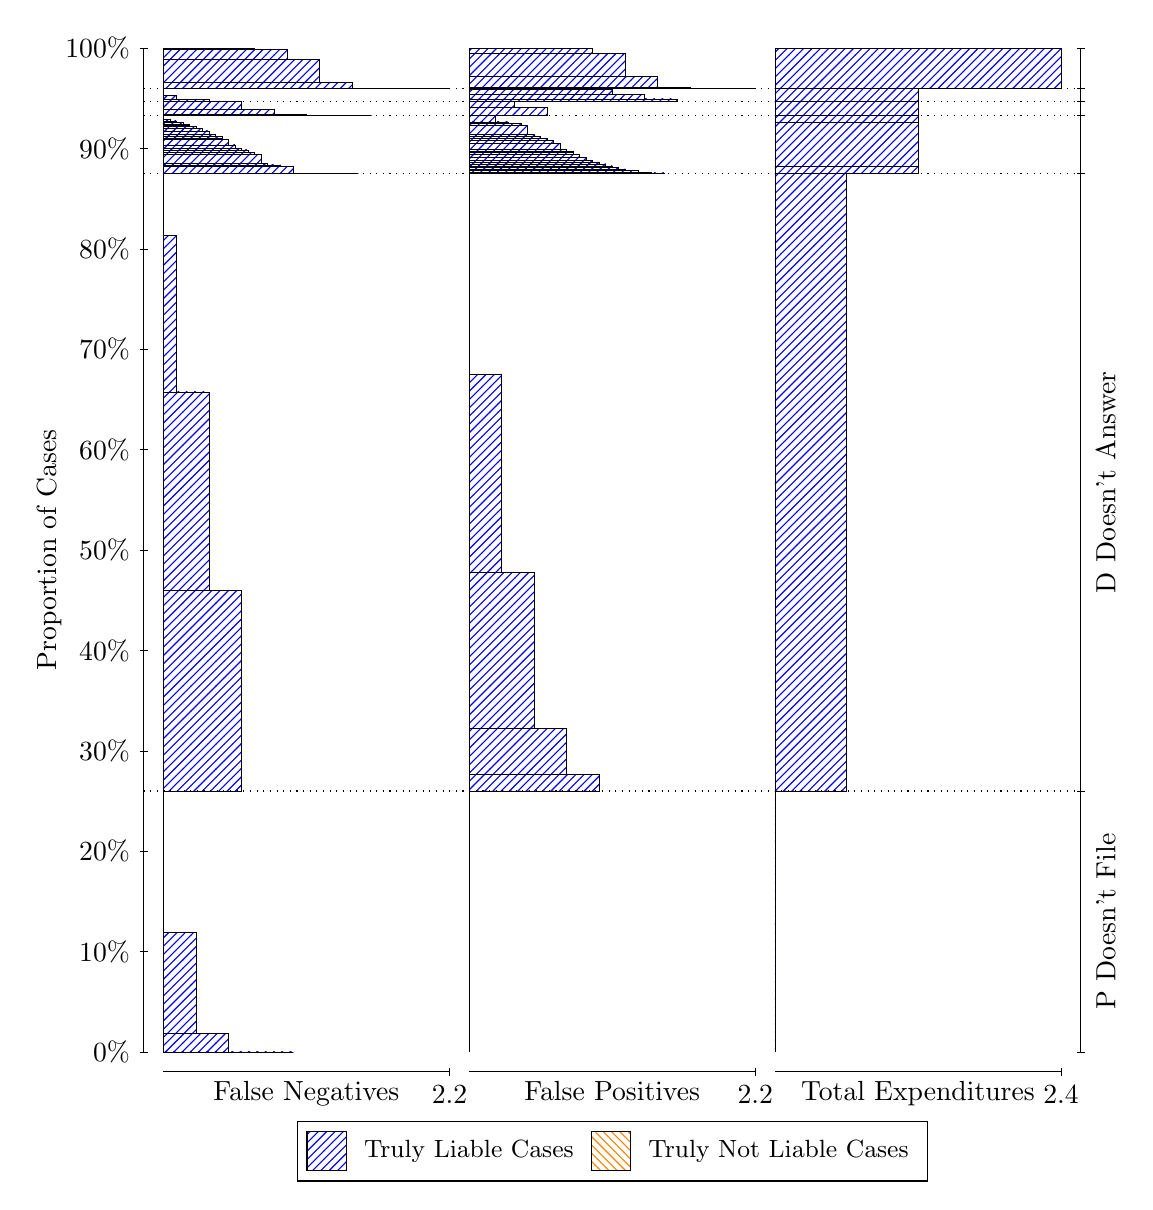
\begin{tikzpicture}
\draw[black, very thin] (1.5,1.75) -- (1.5,14.5);
\node[rotate=90, anchor=center] at (0.3, 8.125) {Proportion of Cases};
\draw[black, very thin] (1.45,1.75) -- (1.55,1.75);
\node[anchor=east] at (1.45, 1.75) {0\%};
\draw[black, very thin] (1.45,3.025) -- (1.55,3.025);
\node[anchor=east] at (1.45, 3.025) {10\%};
\draw[black, very thin] (1.45,4.3) -- (1.55,4.3);
\node[anchor=east] at (1.45, 4.3) {20\%};
\draw[black, very thin] (1.45,5.575) -- (1.55,5.575);
\node[anchor=east] at (1.45, 5.575) {30\%};
\draw[black, very thin] (1.45,6.85) -- (1.55,6.85);
\node[anchor=east] at (1.45, 6.85) {40\%};
\draw[black, very thin] (1.45,8.125) -- (1.55,8.125);
\node[anchor=east] at (1.45, 8.125) {50\%};
\draw[black, very thin] (1.45,9.4) -- (1.55,9.4);
\node[anchor=east] at (1.45, 9.4) {60\%};
\draw[black, very thin] (1.45,10.675) -- (1.55,10.675);
\node[anchor=east] at (1.45, 10.675) {70\%};
\draw[black, very thin] (1.45,11.95) -- (1.55,11.95);
\node[anchor=east] at (1.45, 11.95) {80\%};
\draw[black, very thin] (1.45,13.225) -- (1.55,13.225);
\node[anchor=east] at (1.45, 13.225) {90\%};
\draw[black, very thin] (1.45,14.5) -- (1.55,14.5);
\node[anchor=east] at (1.45, 14.5) {100\%};

\draw[black, very thin] (13.4,1.75) -- (13.4,14.5);
\draw[black, very thin] (13.35,1.75) -- (13.45,1.75);
\node[anchor=west] at (13.35, 1.75) {};
\draw[black, very thin] (13.35,5.0647) -- (13.45,5.0647);
\node[anchor=west] at (13.35, 5.0647) {};
\draw[black, very thin] (13.35,12.908) -- (13.45,12.908);
\node[anchor=west] at (13.35, 12.908) {};
\draw[black, very thin] (13.35,13.647) -- (13.45,13.647);
\node[anchor=west] at (13.35, 13.647) {};
\draw[black, very thin] (13.35,13.824) -- (13.45,13.824);
\node[anchor=west] at (13.35, 13.824) {};
\draw[black, very thin] (13.35,13.988) -- (13.45,13.988);
\node[anchor=west] at (13.35, 13.988) {};
\draw[black, very thin] (13.35,14.5) -- (13.45,14.5);
\node[anchor=west] at (13.35, 14.5) {};

\draw[black, very thin, pattern color=blue, pattern=north east lines] (1.75,1.75) rectangle (3.4015,1.75);
\draw[black, very thin, pattern color=blue, pattern=north east lines] (1.75,1.75) rectangle (2.9886,1.752);
\draw[black, very thin, pattern color=blue, pattern=north east lines] (1.75,1.752) rectangle (2.5758,1.9834);
\draw[black, very thin, pattern color=blue, pattern=north east lines] (1.75,1.9834) rectangle (2.1629,3.2733);
\draw[black, very thin, pattern color=orange, pattern=north west lines] (1.75,3.2733) rectangle (1.75,3.2733);
\draw[black, very thin, pattern color=blue, pattern=north east lines] (1.75,3.2733) rectangle (1.75,5.0647);
\draw[black, very thin, pattern color=blue, pattern=north east lines] (1.75,5.0647) rectangle (2.7409,7.6143);
\draw[black, very thin, pattern color=blue, pattern=north east lines] (1.75,7.6143) rectangle (2.328,10.132);
\draw[black, very thin, pattern color=blue, pattern=north east lines] (1.75,10.132) rectangle (1.9152,12.116);
\draw[black, very thin, pattern color=orange, pattern=north west lines] (1.75,12.116) rectangle (1.75,12.116);
\draw[black, very thin, pattern color=blue, pattern=north east lines] (1.75,12.116) rectangle (1.75,12.908);
\draw[black, very thin, pattern color=blue, pattern=north east lines] (1.75,12.908) rectangle (4.2273,12.908);
\draw[black, very thin, pattern color=blue, pattern=north east lines] (1.75,12.908) rectangle (4.0621,12.908);
\draw[black, very thin, pattern color=blue, pattern=north east lines] (1.75,12.908) rectangle (3.897,12.908);
\draw[black, very thin, pattern color=blue, pattern=north east lines] (1.75,12.908) rectangle (3.8144,12.91);
\draw[black, very thin, pattern color=blue, pattern=north east lines] (1.75,12.91) rectangle (3.7318,12.91);
\draw[black, very thin, pattern color=blue, pattern=north east lines] (1.75,12.91) rectangle (3.6492,12.91);
\draw[black, very thin, pattern color=blue, pattern=north east lines] (1.75,12.91) rectangle (3.5667,12.91);
\draw[black, very thin, pattern color=blue, pattern=north east lines] (1.75,12.91) rectangle (3.4841,12.911);
\draw[black, very thin, pattern color=blue, pattern=north east lines] (1.75,12.911) rectangle (3.4015,12.995);
\draw[black, very thin, pattern color=blue, pattern=north east lines] (1.75,12.995) rectangle (3.3189,12.995);
\draw[black, very thin, pattern color=blue, pattern=north east lines] (1.75,12.995) rectangle (3.2364,12.995);
\draw[black, very thin, pattern color=blue, pattern=north east lines] (1.75,12.995) rectangle (3.2364,13.016);
\draw[black, very thin, pattern color=blue, pattern=north east lines] (1.75,13.016) rectangle (3.1538,13.016);
\draw[black, very thin, pattern color=blue, pattern=north east lines] (1.75,13.016) rectangle (3.0712,13.037);
\draw[black, very thin, pattern color=blue, pattern=north east lines] (1.75,13.037) rectangle (3.0712,13.037);
\draw[black, very thin, pattern color=blue, pattern=north east lines] (1.75,13.037) rectangle (2.9886,13.153);
\draw[black, very thin, pattern color=blue, pattern=north east lines] (1.75,13.153) rectangle (2.9061,13.172);
\draw[black, very thin, pattern color=blue, pattern=north east lines] (1.75,13.172) rectangle (2.8235,13.173);
\draw[black, very thin, pattern color=blue, pattern=north east lines] (1.75,13.173) rectangle (2.8235,13.207);
\draw[black, very thin, pattern color=blue, pattern=north east lines] (1.75,13.207) rectangle (2.7409,13.228);
\draw[black, very thin, pattern color=blue, pattern=north east lines] (1.75,13.228) rectangle (2.6583,13.269);
\draw[black, very thin, pattern color=blue, pattern=north east lines] (1.75,13.269) rectangle (2.6583,13.271);
\draw[black, very thin, pattern color=blue, pattern=north east lines] (1.75,13.271) rectangle (2.5758,13.339);
\draw[black, very thin, pattern color=blue, pattern=north east lines] (1.75,13.339) rectangle (2.4932,13.359);
\draw[black, very thin, pattern color=blue, pattern=north east lines] (1.75,13.359) rectangle (2.4932,13.373);
\draw[black, very thin, pattern color=blue, pattern=north east lines] (1.75,13.373) rectangle (2.4106,13.383);
\draw[black, very thin, pattern color=blue, pattern=north east lines] (1.75,13.383) rectangle (2.4106,13.404);
\draw[black, very thin, pattern color=blue, pattern=north east lines] (1.75,13.404) rectangle (2.328,13.447);
\draw[black, very thin, pattern color=blue, pattern=north east lines] (1.75,13.447) rectangle (2.2455,13.475);
\draw[black, very thin, pattern color=blue, pattern=north east lines] (1.75,13.475) rectangle (2.2455,13.483);
\draw[black, very thin, pattern color=blue, pattern=north east lines] (1.75,13.483) rectangle (2.1629,13.507);
\draw[black, very thin, pattern color=blue, pattern=north east lines] (1.75,13.507) rectangle (2.0803,13.515);
\draw[black, very thin, pattern color=blue, pattern=north east lines] (1.75,13.515) rectangle (2.0803,13.527);
\draw[black, very thin, pattern color=blue, pattern=north east lines] (1.75,13.527) rectangle (1.9977,13.552);
\draw[black, very thin, pattern color=blue, pattern=north east lines] (1.75,13.552) rectangle (1.9152,13.575);
\draw[black, very thin, pattern color=blue, pattern=north east lines] (1.75,13.575) rectangle (1.8326,13.59);
\draw[black, very thin, pattern color=orange, pattern=north west lines] (1.75,13.59) rectangle (1.75,13.59);
\draw[black, very thin, pattern color=blue, pattern=north east lines] (1.75,13.59) rectangle (1.75,13.647);
\draw[black, very thin, pattern color=blue, pattern=north east lines] (1.75,13.647) rectangle (4.3924,13.647);
\draw[black, very thin, pattern color=blue, pattern=north east lines] (1.75,13.647) rectangle (3.9795,13.647);
\draw[black, very thin, pattern color=blue, pattern=north east lines] (1.75,13.647) rectangle (3.5667,13.654);
\draw[black, very thin, pattern color=blue, pattern=north east lines] (1.75,13.654) rectangle (3.1538,13.722);
\draw[black, very thin, pattern color=blue, pattern=north east lines] (1.75,13.722) rectangle (2.7409,13.824);
\draw[black, very thin, pattern color=orange, pattern=north west lines] (1.75,13.824) rectangle (1.75,13.824);
\draw[black, very thin, pattern color=blue, pattern=north east lines] (1.75,13.824) rectangle (2.7409,13.825);
\draw[black, very thin, pattern color=blue, pattern=north east lines] (1.75,13.825) rectangle (2.328,13.843);
\draw[black, very thin, pattern color=blue, pattern=north east lines] (1.75,13.843) rectangle (1.9152,13.902);
\draw[black, very thin, pattern color=orange, pattern=north west lines] (1.75,13.902) rectangle (1.75,13.902);
\draw[black, very thin, pattern color=blue, pattern=north east lines] (1.75,13.902) rectangle (1.75,13.988);
\draw[black, very thin, pattern color=blue, pattern=north east lines] (1.75,13.988) rectangle (5.3833,13.988);
\draw[black, very thin, pattern color=blue, pattern=north east lines] (1.75,13.988) rectangle (4.9705,13.988);
\draw[black, very thin, pattern color=blue, pattern=north east lines] (1.75,13.988) rectangle (4.5576,13.99);
\draw[black, very thin, pattern color=blue, pattern=north east lines] (1.75,13.99) rectangle (4.1447,14.06);
\draw[black, very thin, pattern color=blue, pattern=north east lines] (1.75,14.06) rectangle (3.7318,14.351);
\draw[black, very thin, pattern color=blue, pattern=north east lines] (1.75,14.351) rectangle (3.3189,14.487);
\draw[black, very thin, pattern color=blue, pattern=north east lines] (1.75,14.487) rectangle (2.9061,14.5);
\draw[black, very thin, pattern color=blue, pattern=north east lines] (1.75,14.5) rectangle (2.4932,14.5);
\draw[black, very thin, pattern color=blue, pattern=north east lines] (1.75,14.5) rectangle (2.0803,14.5);
\draw[black, very thin, pattern color=orange, pattern=north west lines] (1.75,14.5) rectangle (1.75,14.5);
\draw[black, very thin, pattern color=orange, pattern=north west lines] (5.6333,1.75) rectangle (5.6333,1.75);
\draw[black, very thin, pattern color=blue, pattern=north east lines] (5.6333,1.75) rectangle (5.6333,5.0647);
\draw[black, very thin, pattern color=orange, pattern=north west lines] (5.6333,5.0647) rectangle (7.2848,5.0647);
\draw[black, very thin, pattern color=blue, pattern=north east lines] (5.6333,5.0647) rectangle (7.2848,5.2787);
\draw[black, very thin, pattern color=blue, pattern=north east lines] (5.6333,5.2787) rectangle (6.872,5.8572);
\draw[black, very thin, pattern color=blue, pattern=north east lines] (5.6333,5.8572) rectangle (6.4591,7.8412);
\draw[black, very thin, pattern color=blue, pattern=north east lines] (5.6333,7.8412) rectangle (6.0462,10.359);
\draw[black, very thin, pattern color=blue, pattern=north east lines] (5.6333,10.359) rectangle (5.6333,12.908);
\draw[black, very thin, pattern color=orange, pattern=north west lines] (5.6333,12.908) rectangle (8.1106,12.908);
\draw[black, very thin, pattern color=blue, pattern=north east lines] (5.6333,12.908) rectangle (8.1106,12.915);
\draw[black, very thin, pattern color=orange, pattern=north west lines] (5.6333,12.915) rectangle (7.9455,12.915);
\draw[black, very thin, pattern color=blue, pattern=north east lines] (5.6333,12.915) rectangle (7.9455,12.924);
\draw[black, very thin, pattern color=orange, pattern=north west lines] (5.6333,12.924) rectangle (7.7803,12.924);
\draw[black, very thin, pattern color=blue, pattern=north east lines] (5.6333,12.924) rectangle (7.7803,12.943);
\draw[black, very thin, pattern color=blue, pattern=north east lines] (5.6333,12.943) rectangle (7.6977,12.95);
\draw[black, very thin, pattern color=orange, pattern=north west lines] (5.6333,12.95) rectangle (7.6152,12.95);
\draw[black, very thin, pattern color=blue, pattern=north east lines] (5.6333,12.95) rectangle (7.6152,12.966);
\draw[black, very thin, pattern color=blue, pattern=north east lines] (5.6333,12.966) rectangle (7.5326,12.98);
\draw[black, very thin, pattern color=orange, pattern=north west lines] (5.6333,12.98) rectangle (7.45,12.98);
\draw[black, very thin, pattern color=blue, pattern=north east lines] (5.6333,12.98) rectangle (7.45,13.004);
\draw[black, very thin, pattern color=blue, pattern=north east lines] (5.6333,13.004) rectangle (7.3674,13.029);
\draw[black, very thin, pattern color=orange, pattern=north west lines] (5.6333,13.029) rectangle (7.2848,13.029);
\draw[black, very thin, pattern color=blue, pattern=north east lines] (5.6333,13.029) rectangle (7.2848,13.049);
\draw[black, very thin, pattern color=blue, pattern=north east lines] (5.6333,13.049) rectangle (7.2023,13.072);
\draw[black, very thin, pattern color=orange, pattern=north west lines] (5.6333,13.072) rectangle (7.1197,13.072);
\draw[black, very thin, pattern color=blue, pattern=north east lines] (5.6333,13.072) rectangle (7.1197,13.108);
\draw[black, very thin, pattern color=blue, pattern=north east lines] (5.6333,13.108) rectangle (7.0371,13.152);
\draw[black, very thin, pattern color=orange, pattern=north west lines] (5.6333,13.152) rectangle (6.9545,13.152);
\draw[black, very thin, pattern color=blue, pattern=north east lines] (5.6333,13.152) rectangle (6.9545,13.172);
\draw[black, very thin, pattern color=blue, pattern=north east lines] (5.6333,13.172) rectangle (6.9545,13.183);
\draw[black, very thin, pattern color=blue, pattern=north east lines] (5.6333,13.183) rectangle (6.872,13.217);
\draw[black, very thin, pattern color=orange, pattern=north west lines] (5.6333,13.217) rectangle (6.7894,13.217);
\draw[black, very thin, pattern color=blue, pattern=north east lines] (5.6333,13.217) rectangle (6.7894,13.285);
\draw[black, very thin, pattern color=blue, pattern=north east lines] (5.6333,13.285) rectangle (6.7068,13.328);
\draw[black, very thin, pattern color=blue, pattern=north east lines] (5.6333,13.328) rectangle (6.6242,13.349);
\draw[black, very thin, pattern color=blue, pattern=north east lines] (5.6333,13.349) rectangle (6.5417,13.383);
\draw[black, very thin, pattern color=blue, pattern=north east lines] (5.6333,13.383) rectangle (6.5417,13.384);
\draw[black, very thin, pattern color=blue, pattern=north east lines] (5.6333,13.384) rectangle (6.4591,13.403);
\draw[black, very thin, pattern color=blue, pattern=north east lines] (5.6333,13.403) rectangle (6.3765,13.519);
\draw[black, very thin, pattern color=blue, pattern=north east lines] (5.6333,13.519) rectangle (6.2939,13.539);
\draw[black, very thin, pattern color=blue, pattern=north east lines] (5.6333,13.539) rectangle (6.2114,13.54);
\draw[black, very thin, pattern color=blue, pattern=north east lines] (5.6333,13.54) rectangle (6.1288,13.56);
\draw[black, very thin, pattern color=blue, pattern=north east lines] (5.6333,13.56) rectangle (6.1288,13.561);
\draw[black, very thin, pattern color=blue, pattern=north east lines] (5.6333,13.561) rectangle (6.0462,13.561);
\draw[black, very thin, pattern color=blue, pattern=north east lines] (5.6333,13.561) rectangle (5.9636,13.645);
\draw[black, very thin, pattern color=blue, pattern=north east lines] (5.6333,13.645) rectangle (5.8811,13.645);
\draw[black, very thin, pattern color=blue, pattern=north east lines] (5.6333,13.645) rectangle (5.7985,13.645);
\draw[black, very thin, pattern color=blue, pattern=north east lines] (5.6333,13.645) rectangle (5.7159,13.646);
\draw[black, very thin, pattern color=blue, pattern=north east lines] (5.6333,13.646) rectangle (5.6333,13.647);
\draw[black, very thin, pattern color=orange, pattern=north west lines] (5.6333,13.647) rectangle (6.6242,13.647);
\draw[black, very thin, pattern color=blue, pattern=north east lines] (5.6333,13.647) rectangle (6.6242,13.75);
\draw[black, very thin, pattern color=blue, pattern=north east lines] (5.6333,13.75) rectangle (6.2114,13.818);
\draw[black, very thin, pattern color=blue, pattern=north east lines] (5.6333,13.818) rectangle (5.7985,13.824);
\draw[black, very thin, pattern color=blue, pattern=north east lines] (5.6333,13.824) rectangle (5.6333,13.824);
\draw[black, very thin, pattern color=orange, pattern=north west lines] (5.6333,13.824) rectangle (8.2758,13.824);
\draw[black, very thin, pattern color=blue, pattern=north east lines] (5.6333,13.824) rectangle (8.2758,13.853);
\draw[black, very thin, pattern color=blue, pattern=north east lines] (5.6333,13.853) rectangle (7.8629,13.911);
\draw[black, very thin, pattern color=blue, pattern=north east lines] (5.6333,13.911) rectangle (7.45,13.97);
\draw[black, very thin, pattern color=blue, pattern=north east lines] (5.6333,13.97) rectangle (7.0371,13.988);
\draw[black, very thin, pattern color=blue, pattern=north east lines] (5.6333,13.988) rectangle (6.6242,13.988);
\draw[black, very thin, pattern color=orange, pattern=north west lines] (5.6333,13.988) rectangle (9.2667,13.988);
\draw[black, very thin, pattern color=blue, pattern=north east lines] (5.6333,13.988) rectangle (9.2667,13.988);
\draw[black, very thin, pattern color=blue, pattern=north east lines] (5.6333,13.988) rectangle (8.8538,13.989);
\draw[black, very thin, pattern color=orange, pattern=north west lines] (5.6333,13.989) rectangle (8.8538,13.989);
\draw[black, very thin, pattern color=blue, pattern=north east lines] (5.6333,13.989) rectangle (8.8538,13.989);
\draw[black, very thin, pattern color=blue, pattern=north east lines] (5.6333,13.989) rectangle (8.4409,13.99);
\draw[black, very thin, pattern color=orange, pattern=north west lines] (5.6333,13.99) rectangle (8.4409,13.99);
\draw[black, very thin, pattern color=blue, pattern=north east lines] (5.6333,13.99) rectangle (8.4409,14.002);
\draw[black, very thin, pattern color=blue, pattern=north east lines] (5.6333,14.002) rectangle (8.028,14.003);
\draw[black, very thin, pattern color=orange, pattern=north west lines] (5.6333,14.003) rectangle (8.028,14.003);
\draw[black, very thin, pattern color=blue, pattern=north east lines] (5.6333,14.003) rectangle (8.028,14.137);
\draw[black, very thin, pattern color=blue, pattern=north east lines] (5.6333,14.137) rectangle (7.6152,14.137);
\draw[black, very thin, pattern color=orange, pattern=north west lines] (5.6333,14.137) rectangle (7.6152,14.137);
\draw[black, very thin, pattern color=blue, pattern=north east lines] (5.6333,14.137) rectangle (7.6152,14.429);
\draw[black, very thin, pattern color=blue, pattern=north east lines] (5.6333,14.429) rectangle (7.2023,14.498);
\draw[black, very thin, pattern color=blue, pattern=north east lines] (5.6333,14.498) rectangle (6.7894,14.5);
\draw[black, very thin, pattern color=blue, pattern=north east lines] (5.6333,14.5) rectangle (6.3765,14.5);
\draw[black, very thin, pattern color=blue, pattern=north east lines] (5.6333,14.5) rectangle (5.9636,14.5);
\draw[black, very thin, pattern color=orange, pattern=north west lines] (9.5167,1.75) rectangle (9.5167,1.75);
\draw[black, very thin, pattern color=blue, pattern=north east lines] (9.5167,1.75) rectangle (9.5167,5.0647);
\draw[black, very thin, pattern color=orange, pattern=north west lines] (9.5167,5.0647) rectangle (10.425,5.0647);
\draw[black, very thin, pattern color=blue, pattern=north east lines] (9.5167,5.0647) rectangle (10.425,12.908);
\draw[black, very thin, pattern color=orange, pattern=north west lines] (9.5167,12.908) rectangle (11.333,12.908);
\draw[black, very thin, pattern color=blue, pattern=north east lines] (9.5167,12.908) rectangle (11.333,12.997);
\draw[black, very thin, pattern color=orange, pattern=north west lines] (9.5167,12.997) rectangle (11.333,12.997);
\draw[black, very thin, pattern color=blue, pattern=north east lines] (9.5167,12.997) rectangle (11.333,13.558);
\draw[black, very thin, pattern color=orange, pattern=north west lines] (9.5167,13.558) rectangle (11.333,13.558);
\draw[black, very thin, pattern color=blue, pattern=north east lines] (9.5167,13.558) rectangle (11.333,13.647);
\draw[black, very thin, pattern color=orange, pattern=north west lines] (9.5167,13.647) rectangle (11.333,13.647);
\draw[black, very thin, pattern color=blue, pattern=north east lines] (9.5167,13.647) rectangle (11.333,13.824);
\draw[black, very thin, pattern color=orange, pattern=north west lines] (9.5167,13.824) rectangle (11.333,13.824);
\draw[black, very thin, pattern color=blue, pattern=north east lines] (9.5167,13.824) rectangle (11.333,13.988);
\draw[black, very thin, pattern color=orange, pattern=north west lines] (9.5167,13.988) rectangle (13.15,13.988);
\draw[black, very thin, pattern color=blue, pattern=north east lines] (9.5167,13.988) rectangle (13.15,13.991);
\draw[black, very thin, pattern color=orange, pattern=north west lines] (9.5167,13.991) rectangle (13.15,13.991);
\draw[black, very thin, pattern color=blue, pattern=north east lines] (9.5167,13.991) rectangle (13.15,14.5);
\draw[black, dotted] (1.5,5.0647) -- (13.4,5.0647);
\draw[black, dotted] (1.5,12.908) -- (13.4,12.908);
\draw[black, dotted] (1.5,13.647) -- (13.4,13.647);
\draw[black, dotted] (1.5,13.824) -- (13.4,13.824);
\draw[black, dotted] (1.5,13.988) -- (13.4,13.988);
\draw[black, very thin] (1.75,1.5) -- (5.3833,1.5);
\node[anchor=north] at (3.5667, 1.5) {False Negatives};
\draw[black, very thin] (5.3833,1.45) -- (5.3833,1.55);
\node[anchor=north] at (5.3833, 1.45) {2.2};

\draw[black, very thin] (5.6333,1.5) -- (9.2667,1.5);
\node[anchor=north] at (7.45, 1.5) {False Positives};
\draw[black, very thin] (9.2667,1.45) -- (9.2667,1.55);
\node[anchor=north] at (9.2667, 1.45) {2.2};

\draw[black, very thin] (9.5167,1.5) -- (13.15,1.5);
\node[anchor=north] at (11.333, 1.5) {Total Expenditures};
\draw[black, very thin] (13.15,1.45) -- (13.15,1.55);
\node[anchor=north] at (13.15, 1.45) {2.4};

\node[black, centered, rotate=90] at (13.72, 3.4073) {P Doesn't File};
\node[black, centered, rotate=90] at (13.72, 8.9865) {D Doesn't Answer};





\draw (7.449999999999999,1.5) node[draw=none] (baseCoordinate) {};
\begin{scope}[align=center]
        \matrix[scale=0.5, draw=black, below=0.5cm of baseCoordinate, nodes={draw}, column sep=0.1cm]{
            \node[rectangle, draw, minimum width=0.5cm, minimum height=0.5cm, pattern=north east lines, pattern color=blue] {}; &
            \node[draw=none, font=\small] (B) {Truly Liable Cases}; &
            \node[rectangle, draw, minimum width=0.5cm, minimum height=0.5cm, pattern=north west lines, pattern color=orange] {}; &
            \node[draw=none, font=\small] (B) {Truly Not Liable Cases}; \\
            };
\end{scope}

\end{tikzpicture}
\end{document}